\chapter{Evaluation}

\section{Dieharder Results}

Dieharder is designed to push the tests to unambiguous failure CITE Robert G. Brown's General Tools Page (duke.edu) . It contains a number of flag options to alter the parameters of the tests and change their acceptance criteria. The command used to run the Dieharder test suite for this project was:\newline

Dieharder -a -k 2 -Y 1 -f <filename>\newline

The -a flag runs all the tests in the dieharder test suite, as described in  section BLANK. The -k flag is the ks-flag K sminorv thing. The -Y flag is the Xtrategy flag which is used to control the ‘test to failure’ modes. CITE  rgb. This flag is set to 1 to use the ‘resolve ambiguity’ mode. Dieharder can return ‘weak’ as a test result which can be difficult to interpret. Even perfect random numbers will return some ‘weak’ results at some point because the p-values are uniformly distributed and will have a result in the tails of the distribution from time to time. Even if a test returns more than one weak result, this is not conclusive evidence that the data is non-random. The ‘resolve ambiguity’ mode resolves this issue by adding p-samples (in blocks of 100) until the test results in a definitive pass, weak or it proceeds to failure. \newline

\subsection{TEKs Results}
Table for teks
\begin{longtable}{cccccc}
\toprule
Test Name & $n$ & $N$ & $d$ & $p$-value & Result \\
\midrule
diehard\_birthdays & 0 & 100 & 100 & 0.77299183 & PASSED \\
diehard\_operm5 & 0 & 1000000 & 100 & 0.13537941 & PASSED \\
diehard\_rank\_32x32 & 0 & 40000 & 100 & 0.07349656 & PASSED \\
diehard\_rank\_6x8 & 0 & 100000 & 100 & 0.14027053 & PASSED \\
diehard\_bitstream & 0 & 2097152 & 100 & 0.74598222 & PASSED \\
diehard\_opso & 0 & 2097152 & 100 & 0.09336658 & PASSED \\
diehard\_oqso & 0 & 2097152 & 100 & 0.85904097 & PASSED \\
diehard\_dna & 0 & 2097152 & 100 & 0.97496850 & PASSED \\
diehard\_count\_1s\_str & 0 & 256000 & 100 & 0.94811453 & PASSED \\
diehard\_count\_1s\_byt & 0 & 256000 & 100 & 0.63133151 & PASSED \\
diehard\_parking\_lot & 0 & 12000 & 100 & 0.48712953 & PASSED \\
diehard\_2dsphere & 2 & 8000 & 100 & 0.61476303 & PASSED \\
diehard\_3dsphere & 3 & 4000 & 100 & 0.62134392 & PASSED \\
diehard\_squeeze & 0 & 100000 & 100 & 0.46769179 & PASSED \\
diehard\_sums & 0 & 100 & 100 & 0.04953850 & PASSED \\
diehard\_runs & 0 & 100000 & 100 & 0.19288118 & PASSED \\
diehard\_runs & 0 & 100000 & 100 & 0.54574717 & PASSED \\
diehard\_craps & 0 & 200000 & 100 & 0.90596413 & PASSED \\
diehard\_craps & 0 & 200000 & 100 & 0.18959393 & PASSED \\
marsaglia\_tsang\_gcd & 0 & 10000000 & 100 & 0.00000000 & FAILED \\
marsaglia\_tsang\_gcd & 0 & 10000000 & 100 & 0.10568644 & PASSED \\
sts\_monobit & 1 & 100000 & 100 & 0.47976313 & PASSED \\
sts\_runs & 2 & 100000 & 100 & 0.66676814 & PASSED \\
sts\_serial & 1 & 100000 & 100 & 0.78623968 & PASSED \\
sts\_serial & 2 & 100000 & 100 & 0.44645002 & PASSED \\
sts\_serial & 3 & 100000 & 100 & 0.43604239 & PASSED \\
sts\_serial & 3 & 100000 & 100 & 0.38891073 & PASSED \\
sts\_serial & 4 & 100000 & 100 & 0.08927189 & PASSED \\
sts\_serial & 4 & 100000 & 100 & 0.45728138 & PASSED \\
sts\_serial & 5 & 100000 & 100 & 0.45061005 & PASSED \\
sts\_serial & 5 & 100000 & 100 & 0.94187841 & PASSED \\
sts\_serial & 6 & 100000 & 100 & 0.74013647 & PASSED \\
sts\_serial & 6 & 100000 & 100 & 0.96963845 & PASSED \\
sts\_serial & 7 & 100000 & 100 & 0.16445098 & PASSED \\
sts\_serial & 7 & 100000 & 100 & 0.39368207 & PASSED \\
sts\_serial & 8 & 100000 & 100 & 0.85303740 & PASSED \\
sts\_serial & 8 & 100000 & 100 & 0.61403945 & PASSED \\
sts\_serial & 9 & 100000 & 100 & 0.82207775 & PASSED \\
sts\_serial & 9 & 100000 & 100 & 0.84023286 & PASSED \\
sts\_serial & 10 & 100000 & 100 & 0.53878704 & PASSED \\
sts\_serial & 10 & 100000 & 100 & 0.50958419 & PASSED \\
sts\_serial & 11 & 100000 & 100 & 0.76365987 & PASSED \\
sts\_serial & 11 & 100000 & 100 & 0.99724672 & WEAK \\
sts\_serial & 12 & 100000 & 100 & 0.10309010 & PASSED \\
sts\_serial & 12 & 100000 & 100 & 0.09075148 & PASSED \\
sts\_serial & 13 & 100000 & 100 & 0.14193034 & PASSED \\
sts\_serial & 13 & 100000 & 100 & 0.39178650 & PASSED \\
sts\_serial & 14 & 100000 & 100 & 0.55235953 & PASSED \\
sts\_serial & 14 & 100000 & 100 & 0.93067829 & PASSED \\
sts\_serial & 15 & 100000 & 100 & 0.87023615 & PASSED \\
sts\_serial & 15 & 100000 & 100 & 0.41580060 & PASSED \\
sts\_serial & 16 & 100000 & 100 & 0.30963945 & PASSED \\
sts\_serial & 16 & 100000 & 100 & 0.24160223 & PASSED \\
sts\_serial & 1 & 100000 & 200 & 0.79166956 & PASSED \\
sts\_serial & 2 & 100000 & 200 & 0.83175687 & PASSED \\
sts\_serial & 3 & 100000 & 200 & 0.06738309 & PASSED \\
sts\_serial & 3 & 100000 & 200 & 0.57296112 & PASSED \\
sts\_serial & 4 & 100000 & 200 & 0.24628902 & PASSED \\
sts\_serial & 4 & 100000 & 200 & 0.44915922 & PASSED \\
sts\_serial & 5 & 100000 & 200 & 0.51469111 & PASSED \\
sts\_serial & 5 & 100000 & 200 & 0.99781703 & WEAK \\
sts\_serial & 6 & 100000 & 200 & 0.32098879 & PASSED \\
sts\_serial & 6 & 100000 & 200 & 0.81131383 & PASSED \\
sts\_serial & 7 & 100000 & 200 & 0.43377863 & PASSED \\
sts\_serial & 7 & 100000 & 200 & 0.83148284 & PASSED \\
sts\_serial & 8 & 100000 & 200 & 0.93537243 & PASSED \\
sts\_serial & 8 & 100000 & 200 & 0.42799745 & PASSED \\
sts\_serial & 9 & 100000 & 200 & 0.93092228 & PASSED \\
sts\_serial & 9 & 100000 & 200 & 0.97411788 & PASSED \\
sts\_serial & 10 & 100000 & 200 & 0.74041098 & PASSED \\
sts\_serial & 10 & 100000 & 200 & 0.57488851 & PASSED \\
sts\_serial & 11 & 100000 & 200 & 0.94741770 & PASSED \\
sts\_serial & 11 & 100000 & 200 & 0.97652870 & PASSED \\
sts\_serial & 12 & 100000 & 200 & 0.36943161 & PASSED \\
sts\_serial & 12 & 100000 & 200 & 0.11761168 & PASSED \\
sts\_serial & 13 & 100000 & 200 & 0.09077406 & PASSED \\
sts\_serial & 13 & 100000 & 200 & 0.65800529 & PASSED \\
sts\_serial & 14 & 100000 & 200 & 0.52298457 & PASSED \\
sts\_serial & 14 & 100000 & 200 & 0.80247788 & PASSED \\
sts\_serial & 15 & 100000 & 200 & 0.15737979 & PASSED \\
sts\_serial & 15 & 100000 & 200 & 0.31245746 & PASSED \\
sts\_serial & 16 & 100000 & 200 & 0.97689150 & PASSED \\
sts\_serial & 16 & 100000 & 200 & 0.35214966 & PASSED \\
sts\_serial & 1 & 100000 & 300 & 0.24837866 & PASSED \\
sts\_serial & 2 & 100000 & 300 & 0.19541588 & PASSED \\
sts\_serial & 3 & 100000 & 300 & 0.05997633 & PASSED \\
sts\_serial & 3 & 100000 & 300 & 0.38771638 & PASSED \\
sts\_serial & 4 & 100000 & 300 & 0.11894101 & PASSED \\
sts\_serial & 4 & 100000 & 300 & 0.47096021 & PASSED \\
sts\_serial & 5 & 100000 & 300 & 0.72546069 & PASSED \\
sts\_serial & 5 & 100000 & 300 & 0.49034451 & PASSED \\
sts\_serial & 6 & 100000 & 300 & 0.22938997 & PASSED \\
sts\_serial & 6 & 100000 & 300 & 0.49108463 & PASSED \\
sts\_serial & 7 & 100000 & 300 & 0.24917545 & PASSED \\
sts\_serial & 7 & 100000 & 300 & 0.52041708 & PASSED \\
sts\_serial & 8 & 100000 & 300 & 0.91268041 & PASSED \\
sts\_serial & 8 & 100000 & 300 & 0.37811375 & PASSED \\
sts\_serial & 9 & 100000 & 300 & 0.72626048 & PASSED \\
sts\_serial & 9 & 100000 & 300 & 0.96132189 & PASSED \\
sts\_serial & 10 & 100000 & 300 & 0.28380339 & PASSED \\
sts\_serial & 10 & 100000 & 300 & 0.18689871 & PASSED \\
sts\_serial & 11 & 100000 & 300 & 0.85779874 & PASSED \\
sts\_serial & 11 & 100000 & 300 & 0.87697717 & PASSED \\
sts\_serial & 12 & 100000 & 300 & 0.25145027 & PASSED \\
sts\_serial & 12 & 100000 & 300 & 0.14601927 & PASSED \\
sts\_serial & 13 & 100000 & 300 & 0.19917059 & PASSED \\
sts\_serial & 13 & 100000 & 300 & 0.41143466 & PASSED \\
sts\_serial & 14 & 100000 & 300 & 0.58145201 & PASSED \\
sts\_serial & 14 & 100000 & 300 & 0.68687169 & PASSED \\
sts\_serial & 15 & 100000 & 300 & 0.79775271 & PASSED \\
sts\_serial & 15 & 100000 & 300 & 0.96087417 & PASSED \\
sts\_serial & 16 & 100000 & 300 & 0.88531337 & PASSED \\
sts\_serial & 16 & 100000 & 300 & 0.81499315 & PASSED \\
\bottomrule
\caption{Dieharder Results of TEKS.}
\label{table}
\end{longtable}

\subsection{Random keys Results}
Table for random value
\begin{longtable}{cccccc}
\toprule
Test Name & $n$ & $N$ & $d$ & $p$-value & Result \\
\midrule
\endhead
diehard\_birthdays & 0 & 100 & 100 & 0.76394892 & PASSED \\
diehard\_operm5 & 0 & 1000000 & 100 & 0.18935905 & PASSED \\
diehard\_rank\_32x32 & 0 & 40000 & 100 & 0.21580801 & PASSED \\
diehard\_rank\_6x8 & 0 & 100000 & 100 & 0.02770416 & PASSED \\
diehard\_bitstream & 0 & 2097152 & 100 & 0.75370418 & PASSED \\
diehard\_opso & 0 & 2097152 & 100 & 0.32644238 & PASSED \\
diehard\_oqso & 0 & 2097152 & 100 & 0.89648137 & PASSED \\
diehard\_dna & 0 & 2097152 & 100 & 0.59449638 & PASSED \\
diehard\_count\_1s\_str & 0 & 256000 & 100 & 0.37707042 & PASSED \\
diehard\_count\_1s\_byt & 0 & 256000 & 100 & 0.38613176 & PASSED \\
diehard\_parking\_lot & 0 & 12000 & 100 & 0.98428899 & PASSED \\
diehard\_2dsphere & 2 & 8000 & 100 & 0.57449647 & PASSED \\
diehard\_3dsphere & 3 & 4000 & 100 & 0.47967697 & PASSED \\
diehard\_squeeze & 0 & 100000 & 100 & 0.02908390 & PASSED \\
diehard\_sums & 0 & 100 & 100 & 0.01302183 & PASSED \\
diehard\_runs & 0 & 100000 & 100 & 0.21268023 & PASSED \\
diehard\_runs & 0 & 100000 & 100 & 0.48718248 & PASSED \\
diehard\_craps & 0 & 200000 & 100 & 0.43589180 & PASSED \\
diehard\_craps & 0 & 200000 & 100 & 0.48427891 & PASSED \\
marsaglia\_tsang\_gcd & 0 & 10000000 & 100 & 0.39544378 & PASSED \\
marsaglia\_tsang\_gcd & 0 & 10000000 & 100 & 0.00073901 & WEAK \\
marsaglia\_tsang\_gcd & 0 & 10000000 & 200 & 0.20103622 & PASSED \\
marsaglia\_tsang\_gcd & 0 & 10000000 & 200 & 0.00000116 & WEAK \\
marsaglia\_tsang\_gcd & 0 & 10000000 & 300 & 0.15296148 & PASSED \\
marsaglia\_tsang\_gcd & 0 & 10000000 & 300 & 0.00000000 & FAILED \\
sts\_monobit & 1 & 100000 & 100 & 0.46954912 & PASSED \\
sts\_runs & 2 & 100000 & 100 & 0.99997882 & WEAK \\
sts\_runs & 2 & 100000 & 200 & 0.65262205 & PASSED \\
sts\_serial & 1 & 100000 & 100 & 0.75039800 & PASSED \\
sts\_serial & 2 & 100000 & 100 & 0.46782328 & PASSED \\
sts\_serial & 3 & 100000 & 100 & 0.96422500 & PASSED \\
sts\_serial & 3 & 100000 & 100 & 0.38336381 & PASSED \\
sts\_serial & 4 & 100000 & 100 & 0.78436629 & PASSED \\
sts\_serial & 4 & 100000 & 100 & 0.32790423 & PASSED \\
sts\_serial & 5 & 100000 & 100 & 0.93561180 & PASSED \\
sts\_serial & 5 & 100000 & 100 & 0.78894832 & PASSED \\
sts\_serial & 6 & 100000 & 100 & 0.30162394 & PASSED \\
sts\_serial & 6 & 100000 & 100 & 0.45041009 & PASSED \\
sts\_serial & 7 & 100000 & 100 & 0.60514729 & PASSED \\
sts\_serial & 7 & 100000 & 100 & 0.52470608 & PASSED \\
sts\_serial & 8 & 100000 & 100 & 0.38468429 & PASSED \\
sts\_serial & 8 & 100000 & 100 & 0.97346520 & PASSED \\
sts\_serial & 9 & 100000 & 100 & 0.67677659 & PASSED \\
sts\_serial & 9 & 100000 & 100 & 0.21257824 & PASSED \\
sts\_serial & 10 & 100000 & 100 & 0.06065198 & PASSED \\
sts\_serial & 10 & 100000 & 100 & 0.19676120 & PASSED \\
sts\_serial & 11 & 100000 & 100 & 0.25074198 & PASSED \\
sts\_serial & 11 & 100000 & 100 & 0.44324414 & PASSED \\
sts\_serial & 12 & 100000 & 100 & 0.06981655 & PASSED \\
sts\_serial & 12 & 100000 & 100 & 0.26688079 & PASSED \\
sts\_serial & 13 & 100000 & 100 & 0.50138141 & PASSED \\
sts\_serial & 13 & 100000 & 100 & 0.51148391 & PASSED \\
sts\_serial & 14 & 100000 & 100 & 0.38406027 & PASSED \\
sts\_serial & 14 & 100000 & 100 & 0.32968726 & PASSED \\
sts\_serial & 15 & 100000 & 100 & 0.20468696 & PASSED \\
sts\_serial & 15 & 100000 & 100 & 0.21397465 & PASSED \\
sts\_serial & 16 & 100000 & 100 & 0.16604967 & PASSED \\
sts\_serial & 16 & 100000 & 100 & 0.60748515 & PASSED \\
rgb\_bitdist & 1 & 100000 & 100 & 0.36452077 & PASSED \\
rgb\_bitdist & 2 & 100000 & 100 & 0.94306987 & PASSED \\
rgb\_bitdist & 3 & 100000 & 100 & 0.80290189 & PASSED \\
rgb\_bitdist & 4 & 100000 & 100 & 0.29185388 & PASSED \\
rgb\_bitdist & 5 & 100000 & 100 & 0.69257767 & PASSED \\
rgb\_bitdist & 6 & 100000 & 100 & 0.95139967 & PASSED \\
rgb\_bitdist & 7 & 100000 & 100 & 0.57919220 & PASSED \\
rgb\_bitdist & 8 & 100000 & 100 & 0.45468153 & PASSED \\
rgb\_bitdist & 9 & 100000 & 100 & 0.14850293 & PASSED \\
rgb\_bitdist & 10 & 100000 & 100 & 0.54937469 & PASSED \\
rgb\_bitdist & 11 & 100000 & 100 & 0.28545144 & PASSED \\
rgb\_bitdist & 12 & 100000 & 100 & 0.99636354 & WEAK \\
rgb\_bitdist & 12 & 100000 & 200 & 0.29765398 & PASSED \\
rgb\_minimum\_distance & 2 & 10000 & 1000 & 0.99960225 & WEAK \\
rgb\_minimum\_distance & 2 & 10000 & 1100 & 0.99544792 & WEAK \\
rgb\_minimum\_distance & 2 & 10000 & 1200 & 0.99960423 & WEAK \\
rgb\_minimum\_distance & 2 & 10000 & 1300 & 0.76490064 & PASSED \\
rgb\_minimum\_distance & 3 & 10000 & 1000 & 0.88490597 & PASSED \\
rgb\_minimum\_distance & 4 & 10000 & 1000 & 0.56548230 & PASSED \\
rgb\_minimum\_distance & 5 & 10000 & 1000 & 0.84433241 & PASSED \\
rgb\_permutations & 2 & 100000 & 100 & 0.81514673 & PASSED \\
rgb\_permutations & 3 & 100000 & 100 & 0.86382468 & PASSED \\
rgb\_permutations & 4 & 100000 & 100 & 0.99152004 & PASSED \\
rgb\_permutations & 4 & 100000 & 100 & 0.99152004 & PASSED \\
rgb\_permutations & 5 & 100000 & 100 & 0.31316379 & PASSED \\
rgb\_lagged\_sum & 0 & 1000000 & 100 & 0.26035279 & PASSED \\
rgb\_lagged\_sum & 1 & 1000000 & 100 & 0.99920642 & WEAK \\
rgb\_lagged\_sum & 1 & 1000000 & 200 & 0.29519499 & PASSED \\
rgb\_lagged\_sum & 2 & 1000000 & 100 & 0.28259248 & PASSED \\
rgb\_lagged\_sum & 3 & 1000000 & 100 & 0.99684866 & WEAK \\
rgb\_lagged\_sum & 3 & 1000000 & 200 & 0.75546305 & PASSED \\
rgb\_lagged\_sum & 4 & 1000000 & 100 & 0.97658438 & PASSED \\
rgb\_lagged\_sum & 5 & 1000000 & 100 & 0.44382799 & PASSED \\
rgb\_lagged\_sum & 6 & 1000000 & 100 & 0.97652946 & PASSED \\
rgb\_lagged\_sum & 7 & 1000000 & 100 & 0.87715734 & PASSED \\
rgb\_lagged\_sum & 8 & 1000000 & 100 & 0.42657999 & PASSED \\
rgb\_lagged\_sum & 9 & 1000000 & 100 & 0.32151735 & PASSED \\
rgb\_lagged\_sum & 10 & 1000000 & 100 & 0.48476972 & PASSED \\
rgb\_lagged\_sum & 11 & 1000000 & 100 & 0.94092042 & PASSED \\
rgb\_lagged\_sum & 12 & 1000000 & 100 & 0.72099398 & PASSED \\
rgb\_lagged\_sum & 13 & 1000000 & 100 & 0.81002140 & PASSED \\
rgb\_lagged\_sum & 14 & 1000000 & 100 & 0.15611012 & PASSED \\
rgb\_lagged\_sum & 15 & 1000000 & 100 & 0.92648578 & PASSED \\
rgb\_lagged\_sum & 16 & 1000000 & 100 & 0.78312121 & PASSED \\
rgb\_lagged\_sum & 17 & 1000000 & 100 & 0.48839571 & PASSED \\
rgb\_lagged\_sum & 18 & 1000000 & 100 & 0.52741490 & PASSED \\
rgb\_lagged\_sum & 19 & 1000000 & 100 & 0.57382712 & PASSED \\
rgb\_lagged\_sum & 20 & 1000000 & 100 & 0.73919893 & PASSED \\
rgb\_lagged\_sum & 21 & 1000000 & 100 & 0.72509541 & PASSED \\
rgb\_lagged\_sum & 22 & 1000000 & 100 & 0.41689814 & PASSED \\
rgb\_lagged\_sum & 23 & 1000000 & 100 & 0.60260730 & PASSED \\
rgb\_lagged\_sum & 24 & 1000000 & 100 & 0.90147593 & PASSED \\
rgb\_lagged\_sum & 25 & 1000000 & 100 & 0.40242266 & PASSED \\
rgb\_lagged\_sum & 26 & 1000000 & 100 & 0.73316626 & PASSED \\
rgb\_lagged\_sum & 27 & 1000000 & 100 & 0.97377935 & PASSED \\
rgb\_lagged\_sum & 28 & 1000000 & 100 & 0.40299842 & PASSED \\
rgb\_lagged\_sum & 29 & 1000000 & 100 & 0.55415146 & PASSED \\
rgb\_lagged\_sum & 30 & 1000000 & 100 & 0.91395113 & PASSED \\
rgb\_lagged\_sum & 31 & 1000000 & 100 & 0.59378537 & PASSED \\
rgb\_lagged\_sum & 32 & 1000000 & 100 & 0.57760364 & PASSED \\
rgb\_kstest\_test & 0 & 10000 & 1000 & 0.12119363 & PASSED \\
dab\_bytedistrib & 0 & 51200000 & 1 & 0.79112485 & PASSED \\
dab\_dct & 256 & 50000 & 1 & 0.55110228 & PASSED \\
dab\_filltree & 32 & 15000000 & 1 & 0.55562237 & PASSED \\
dab\_filltree & 32 & 15000000 & 1 & 0.93018984 & PASSED \\
dab\_filltree2 & 0 & 5000000 & 1 & 0.48358687 & PASSED \\
dab\_filltree2 & 1 & 5000000 & 1 & 0.66316672 & PASSED \\
dab\_monobit2 & 12 & 65000000 & 1 & 0.85585632 & PASSED \\
\bottomrule
\caption{Dieharder Results of Random keys.}
\label{table}
\end{longtable}

\section{Other Test Results}

\subsubsection{Plot of Counts}
\begin{figure}[h]
\caption{Plot of Counts for TEKs}
\centering
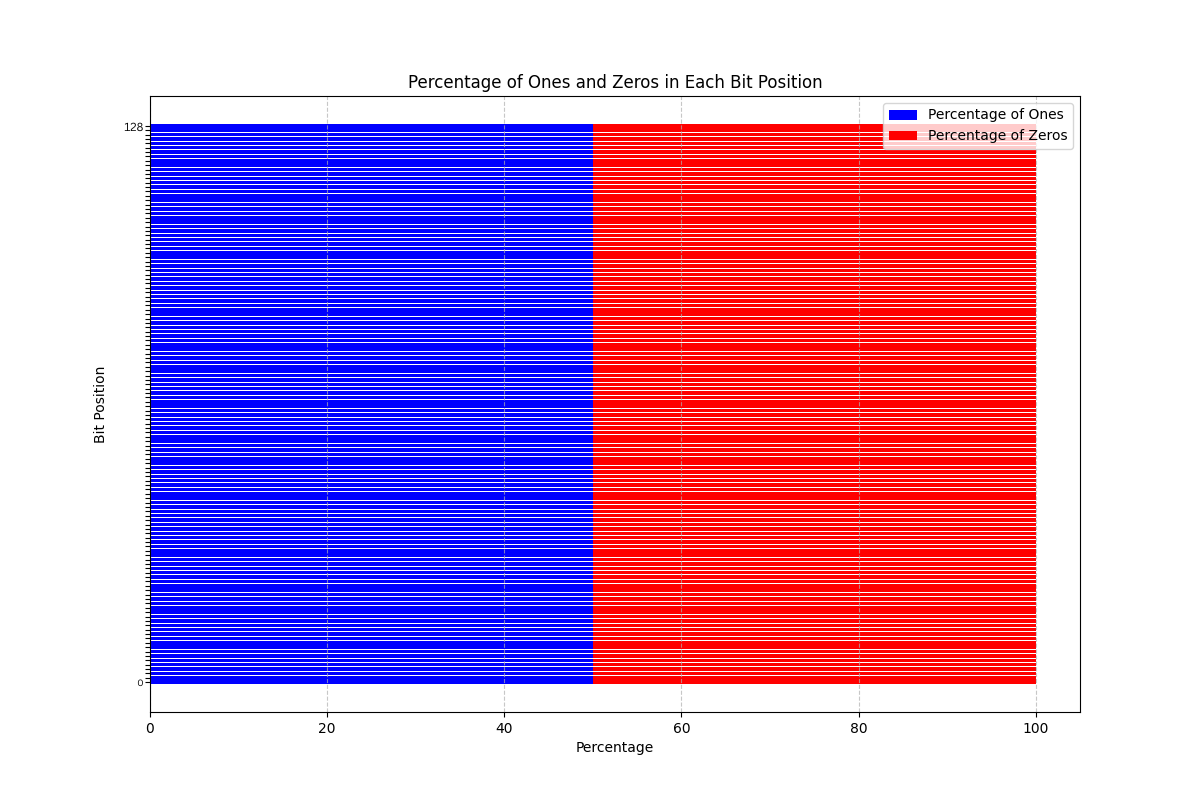
\includegraphics[width=0.5\textwidth]{final0s1sboth.png}
\end{figure}

\begin{figure}[h]
\caption{Plot of Counts for random keys}
\centering
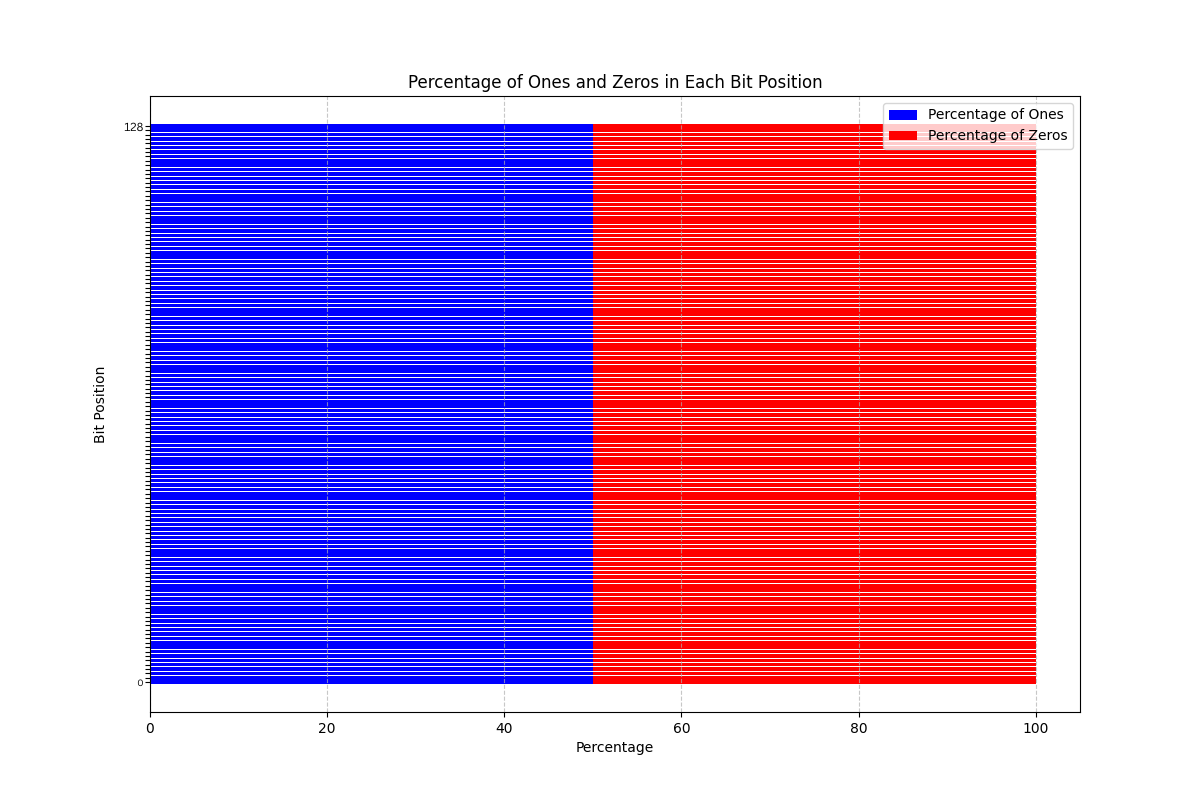
\includegraphics[width=0.5\textwidth]{final0s1sboth.png}
\end{figure}

\subsection{Hilbert Curve}

\subsection{Chi-squared Test}

\subsection{Spectral Test}

\subsection{Lag Plot}
\section{Conclusions}